\begin{frame}{Análisis de la resultados obtenidos en el MCB}
\begin{itemize}

	\item Los resultados obtenidos durante la fase de evaluación para las arquitecturas del MCB han sido mejores que los obtenidos durante la fase de entrenamiento.
	\item Destaca la ausencia de la arquitectura MCB49 entre las cinco configuraciones con mejores resultados del MCB. Este hecho puede atribuirse a factores aleatorios no controlables.
\end{itemize}
	\begin{figure}[H]
    \centering
    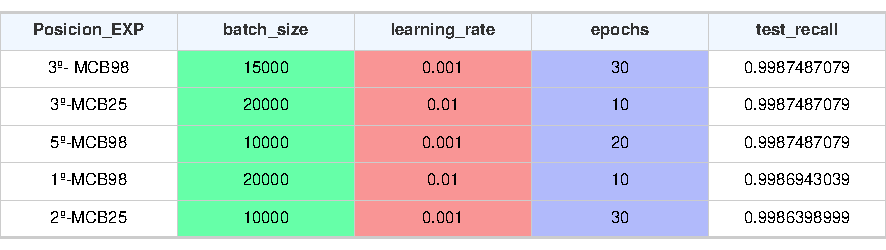
\includegraphics[width=0.9\textwidth]{../Memoria/img/evaluacion/resultados/top5EVALMCB.pdf}
    \caption{Mejores cinco modelos en la fase de evaluación del modelo de clasificación binaria.}
    \label{fig:top5EVALMCB}
\end{figure}
\end{frame}


\begin{frame}{Análisis de la resultados obtenidos en el MCM}
\begin{itemize}

	\item Los resultados obtenidos durante la fase de evaluación para las arquitecturas del MCM han sido ligeramente peores que los obtenidos durante la fase de entrenamiento.
	\item En la fase de evaluación la arquitectura MCB25 ha obtenido un resultado superior respecto al resto de las arquitecturas en comparación con los resultados de la fase de entrenamiento.
\end{itemize}
	\begin{figure}[H]
    \centering
    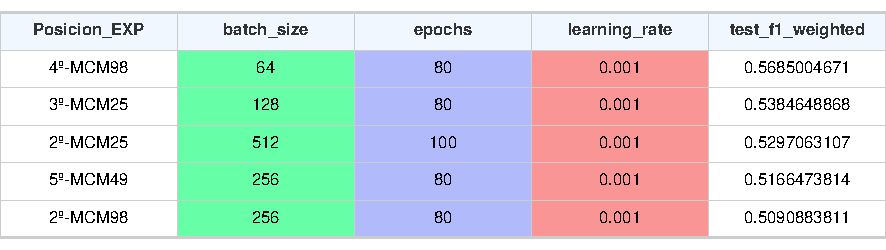
\includegraphics[width=0.9\textwidth]{../Memoria/img/evaluacion/resultados/top5EVALMCM.pdf}
    \caption{Mejores cinco modelos en la fase de evaluación del modelo de clasificación multiclase.}
    \label{fig:top5EVALMCB}
\end{figure}
\end{frame}

\begin{frame}{Matriz de confusión del MCM98 normalizada}
Dado el desbalanceo existente entre el número de muestras de cada clase del conjunto de datos utilizado, es recomendable aplicar la técnica de normalización de la matriz de confusión.% Esta técnica permite observar de forma más clara el comportamiento del modelo en cada clase, independientemente de su frecuencia en los datos. Para ello, se convierten los conteos absolutos de la matriz de confusión en proporciones por cada clase real.


\begin{figure}[H]
    \centering
    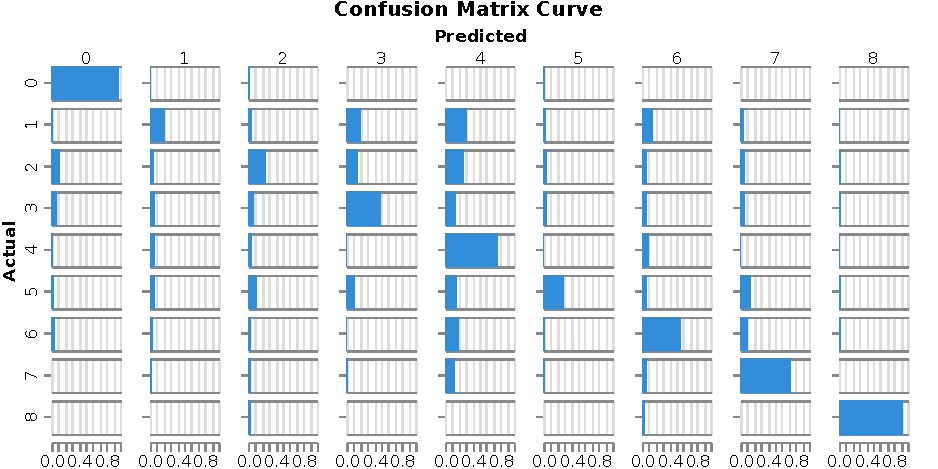
\includegraphics[width=0.95\textwidth]{../Memoria/img/evaluacion/matrices_confusion/MCNorm_EVAL_MCM98.pdf}
    \caption{Matriz de confusión normalizada de la mejor configuración de hiperparámetros obtenida en el MCM98 durante la fase de evaluación.}
    \label{fig:MCNorm_EVAL_MCM98}
\end{figure}

\end{frame}


\begin{frame}{Comparación de los resultados con otros modelos}

Los modelos desarrollados en este trabajo presentan mejoras notables en la clasificación binaria y un rendimiento competitivo en la clasificación multiclase frente a otros modelos publicados anteriormente.% Aunque persisten desafíos en algunas clases, los resultados sugieren una mayor capacidad de generalización frente a los modelos publicados previamente.


\begin{table}[H]
\centering
\resizebox{0.8\textwidth}{!}{
\begin{tabular}{|l|c|c|c|c|c|c|}
\hline
\textbf{Modelo} & \textbf{\textit{Accuracy}} & \textbf{\textit{AUC}} & \textbf{\textit{F1-Score}} & \textbf{\textit{Recall}} & \textbf{\textit{Precision}} & \textbf{\textit{Specificity}} \\
\hline
\textit{Sarhan et al.} & 98.62\% & 0.9485 & 0.85 & -- & -- & -- \\
3º-MCB98 & 99.98\% & 0.9998 & 0.9979 & 0.9987 & 0.9971 & 0.9999 \\
\hline
\end{tabular}
}
\caption{Comparación de modelos de clasificación binaria.}
\label{tab:compbin}
\end{table}


\begin{table}[H]
\centering
\resizebox{0.8\textwidth}{!}{
\begin{tabular}{|l|c|c|}
\hline
\textbf{Clase} & \textbf{\textit{F1-Score} (\textit{Sarhan et al.})} & \textbf{\textit{F1-Score} (4º-MCM98)} \\
\hline
Analysis (0) & 0.15 & 0.97 \\
Backdoor (1) & 0.17 & 0.20 \\
DoS (2) & 0.41 & 0.25 \\
Exploits (3) & 0.82 & 0.48 \\
Fuzzers (4) & 0.55 & 0.75 \\
Generic (5) & 0.66 & 0.28 \\
Reconnaissance (6) & 0.82 & 0.56 \\
Shellcode (7) & 0.75 & 0.72 \\
Worms (8) & 0.55 & 0.92 \\
\hline
\end{tabular}
}
\caption{Comparación de los valores obtenidos en \textit{F1-Score} por clase.}
\label{tab:compmulclass}
\end{table}

\end{frame}



